\beginsong{Kaperslied}[txt={Gottfried Wolters, 1951}, mel={aus Flandern}, bo={12}, pfii={108}, index={Alle, die mit uns auf Kaperfahrt fahren}]

\markboth{\songtitle}{\songtitle}

\beginverse
\endverse

\centering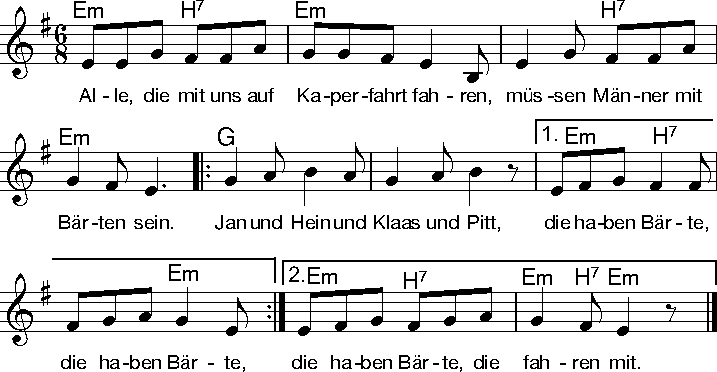
\includegraphics[width=1\textwidth]{Noten/Lied058.pdf}	

\beginverse
\[Em]Alle, die \[H7]Tod und \[Em]Teufel nicht fürchten,
müssen \[H7]Männer mit \[Em]Bärten sein.
\endverse

\beginchorus
\[G]Jan und Hein und Klaas und Pitt,
\[Em]die haben \[H7]Bärte, die haben \[Em]Bärte,
\[G]Jan und Hein und Klaas und Pitt,
\[Em]die haben \[H7]Bärte, die \[Em]fah\[H7]ren \[Em]mit.
\endchorus

\beginverse 
^Alle, die ^Weiber und ^Branntwein lieben,
müssen ^Männer mit ^Bärten sein.
\endverse
\renewcommand{\everychorus}{\textnote{\bf Refrain (wdh.)}}

\beginchorus
\endchorus

\beginverse
^Alle, die ^mit uns das ^Walross schlachten,
müssen ^Männer mit ^Bärten sein.
\endverse

\beginchorus
\endchorus

\beginverse
^Alle, die ^öligen ^Zwieback kauen,
müssen ^Männer mit ^Bärten sein.
\endverse

\beginchorus
\endchorus

\beginverse
^Alle, die ^endlich zur ^Höll' mitfahren,
müssen ^Männer mit ^Bärten sein.
\endverse

\beginchorus
\endchorus

\endsong

\beginscripture{}
%nichts
\endscripture

\begin{intersong}

\end{intersong}